\subsection{\textbf{Future Research}}
\begin{wrapfigure}{r}{110pt}
    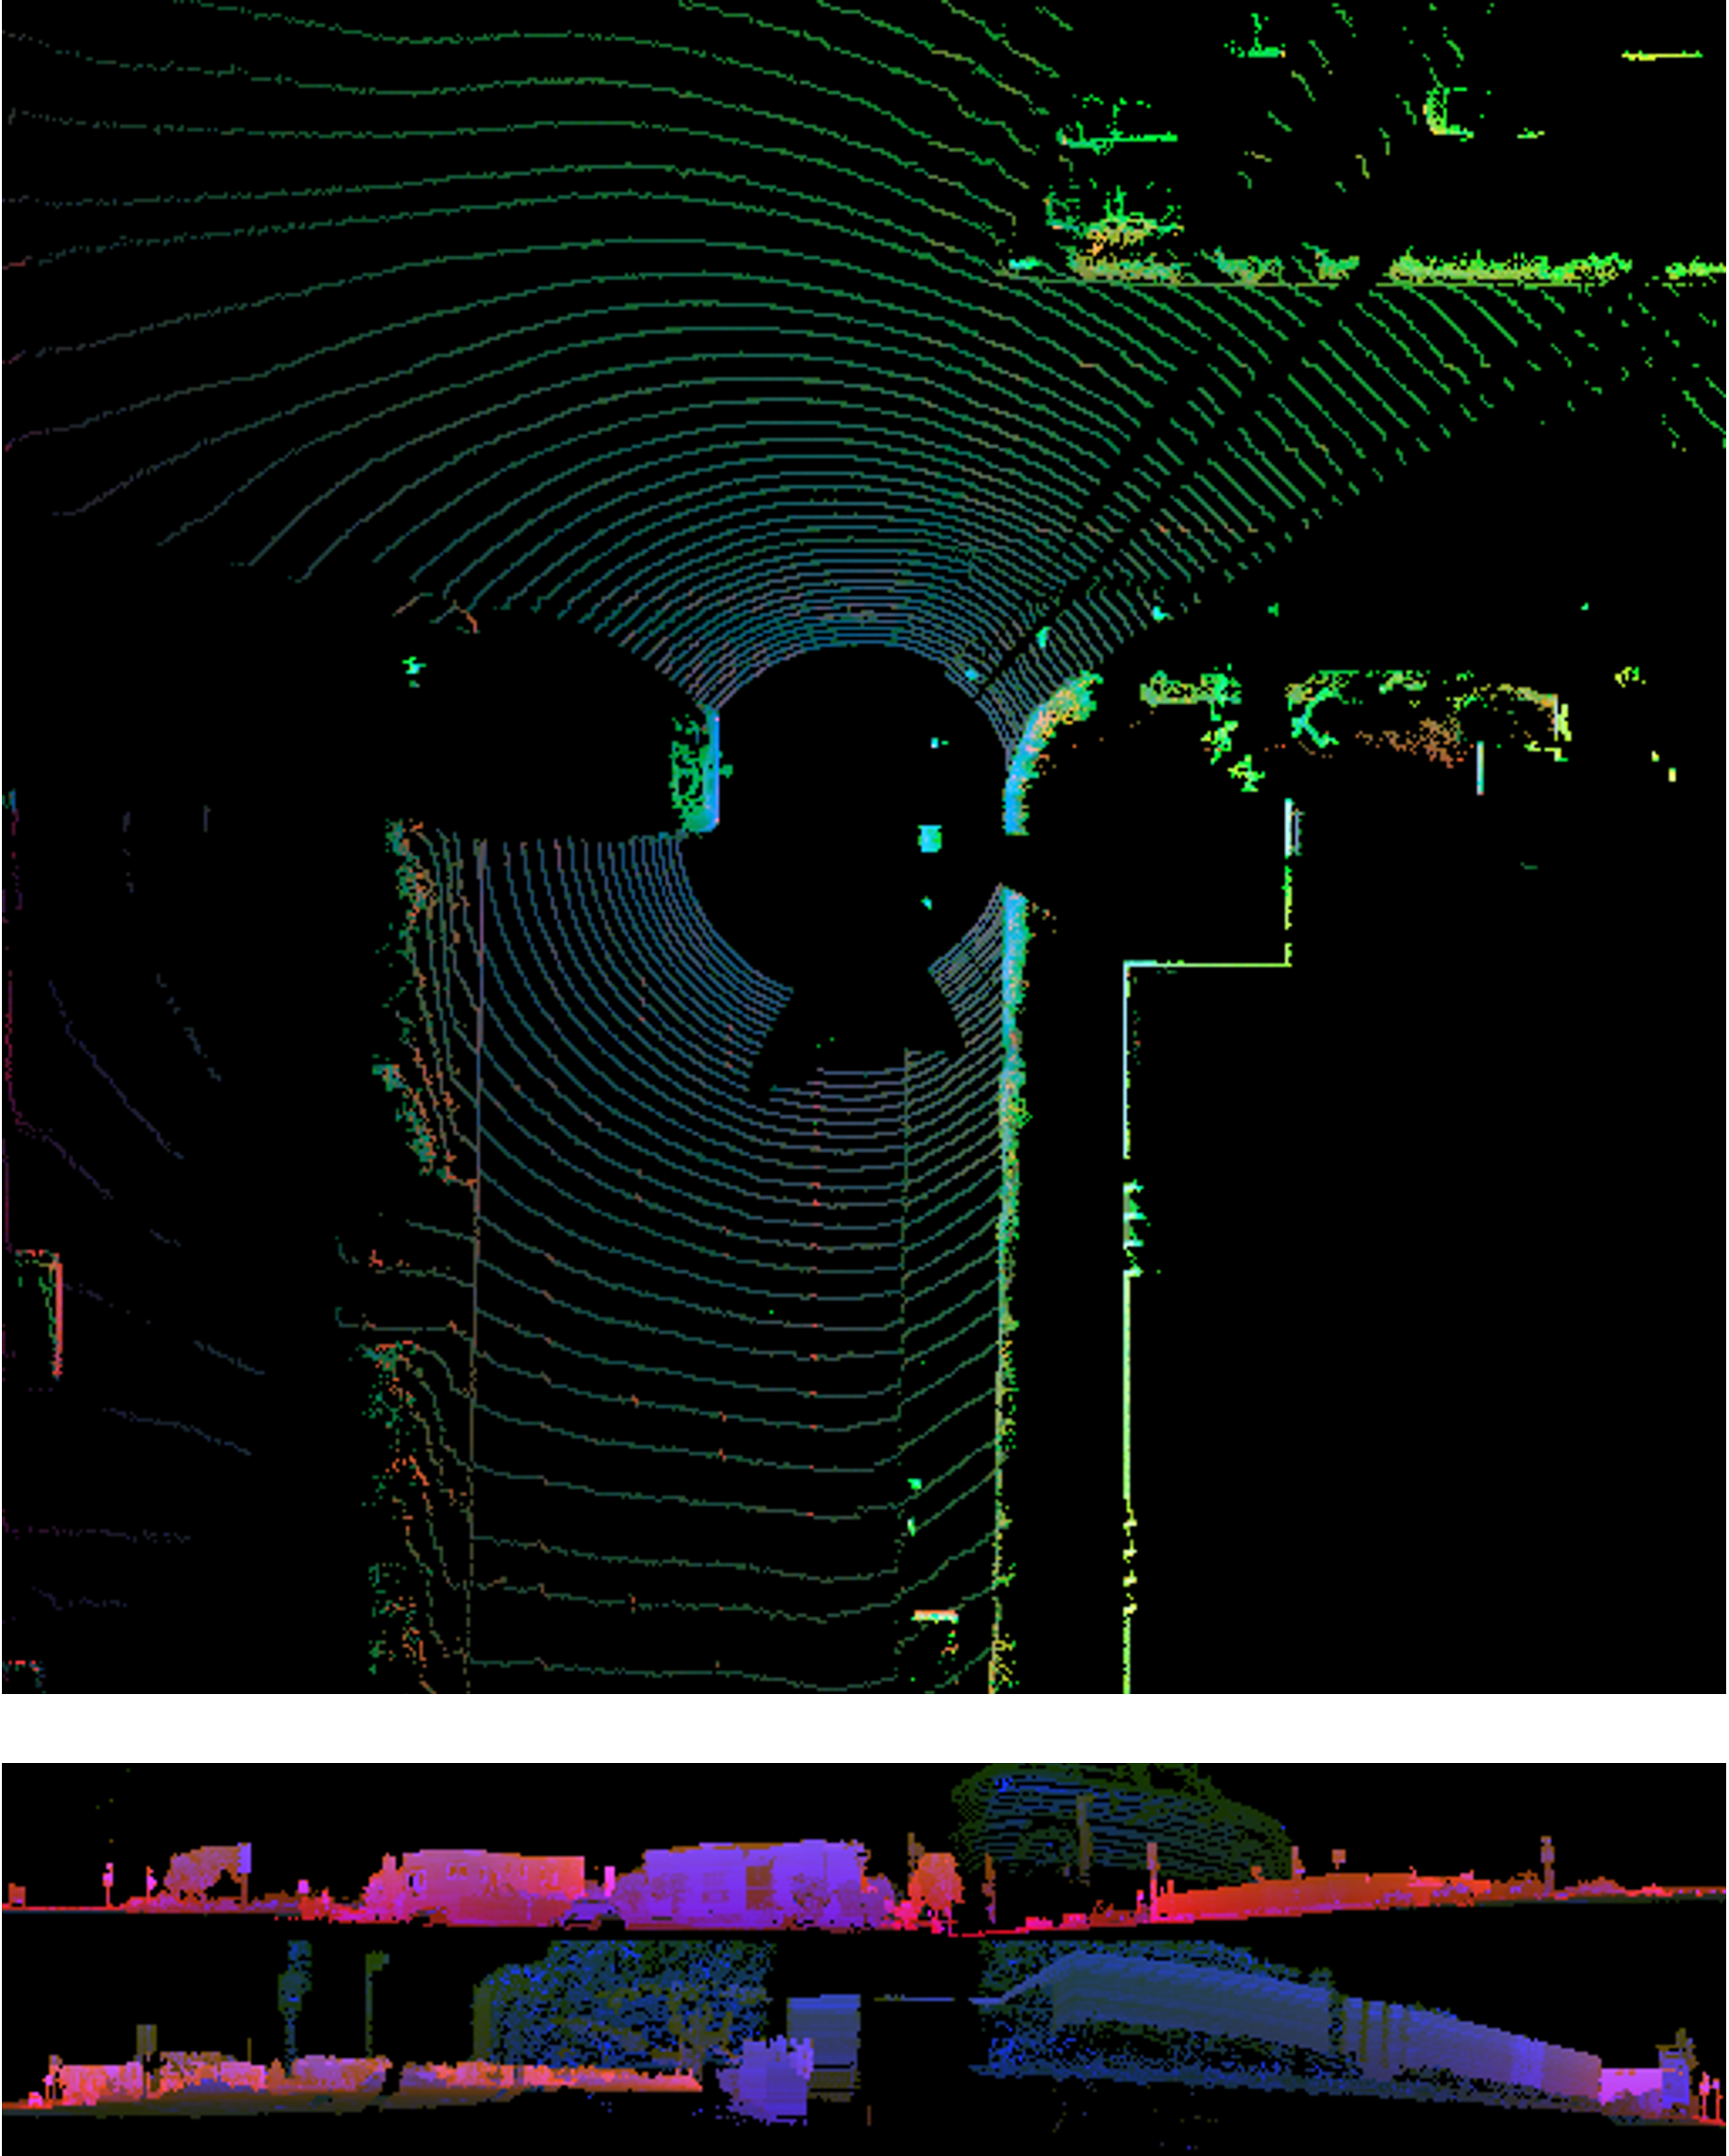
\includegraphics[width=110pt]{pic/fusion.png}
    \mainfont\fontsize{9pt}{9pt}\selectfont\caption{ \mainfont\fontsize{9pt}{9pt}\selectfont Multi view fusion with bird's eye view and spherical view}
    \label{fig:fusion}
    \end{wrapfigure}
In the future, I plan to continue my research in computer vision especially scene understanding and perception while broadening my focus to explore new fields outside of object detection. I am keen to not only explore the possibilities of masked modeling, but also other self-supervised and semi supervised learning techniques.  

The development of pixelNeRF \cite{pixelnerf} opened the line of research of using NeRFs for conditioned scene rendering. With the development of 3D Gaussian splatting and recently methods such as MVSplat \cite{mvsplat} 3D Gaussian representations are obtained with only one forward pass while also rendered in real-time. The 3D Gaussians are a unique latent space for 3D scene representations with many new research avenues to explore. For example the authors of S4C \cite{s4c} use a NeRF to perform 3D semantic scene completion without the need for 3D annotations in a self-supervised manner. I am interested in developing similar methods that make use of the fast rendering of 3D Gaussians for scene understanding.

Methododically I am particular interested in developing and focusing on training strategies such as regularizing via multi task and curriculum learning. For example the authors of ProFusion3D \cite{valada} showcase an impressive multimodal fusion pipeline, while they also focus on novel training strategies via additional objectives in the pretraining phase. 